\section{Results}

This section presents the results obtained from applying various machine learning models to the three different versions of the dataset: the full feature set, the PCA-reduced set, and the feature-selected set. It includes an analysis of performance metrics for each configuration.

\subsection{Model Performance on Full Dataset}

The cross-validated results reported in Table~\ref{tab:cv_performance_fd} highlight the performance of the models when evaluated on the full dataset using repeated stratified k-fold cross-validation. They show the mean and standard deviation (Std) of each metric. Among all models, the \textbf{Random Forest} consistently achieved the best performance across all metrics, demonstrating robustness and generalization ability.
\noindent
The results obtained on the held-out test set, summarized in Table~\ref{tab:test_performance_fd}, confirm the trends observed during cross-validation. Again, the Random Forest classifier slightly outperformed the others, showing balanced precision and recall.
\noindent
While the initial results can be considered moderate (not particularly poor, but not outstanding either), I proceed by applying feature selection to investigate whether performance can be enhanced. These methods aim to reduce noise, remove redundant or irrelevant features, and highlight the most informative dimensions of the data. By simplifying the feature space, I hope to improve model generalization, reduce overfitting, and ultimately increase predictive accuracy and robustness on unseen data.



\begin{table}[ht]
\centering
\caption{Cross-validated performance on the full dataset}
\label{tab:cv_performance_fd}
\renewcommand{\arraystretch}{1.2}
\begin{tabular}{lcccccccc}
\hline
\textbf{Model} & \multicolumn{2}{c}{\textbf{Accuracy}} & \multicolumn{2}{c}{\textbf{F1 Score}} & \multicolumn{2}{c}{\textbf{Recall}} & \multicolumn{2}{c}{\textbf{Precision}} \\
 & Mean & Std & Mean & Std & Mean & Std & Mean & Std \\
\hline
Decision Tree & 0.6210 & 0.0069 & 0.6102 & 0.0065 & 0.6210 & 0.0069 & 0.6216 & 0.0079 \\
\textbf{Random Forest} & \textbf{0.6330} & \textbf{0.0103} & \textbf{0.6197} & \textbf{0.0.121} & \textbf{0.6330} & \textbf{0.0103} & \textbf{0.6743} & \textbf{0.0105} \\
KNN & 0.5653 & 0.0061 & 0.5591 & 0.0064 & 0.5653 & 0.0061 & 0.5611 & 0.0065 \\
Logistic Regression & 0.6173 & 0.0123 & 0.5952 & 0.0136 & 0.6173 & 0.0123 & 0.6252 & 0.0146 \\
Bernoulli Naive Bayes & 0.6056 & 0.0095 & 0.5676 & 0.0116 & 0.6056 & 0.0095 & 0.6236 & 0.0126 \\
\hline
\end{tabular}
\end{table}

\begin{table}[ht]
\centering
\caption{Test performance on the full dataset}
\label{tab:test_performance_fd}
\begin{tabular}{lcccc}
\toprule
\textbf{Model} & \textbf{Accuracy} & \textbf{F1 Score} & \textbf{Recall} & \textbf{Precision} \\
\midrule
Decision Tree & 0.6291 & 0.6188 & 0.6291 & 0.6303 \\
\textbf{Random Forest} & \textbf{0.6318} & \textbf{0.6188} & \textbf{0.6318} & \textbf{0.6353} \\
KNN & 0.5770 & 0.5696 & 0.5770 & 0.5732 \\
Logistic Regression & 0.6146 & 0.5943 & 0.6146 & 0.6203 \\
Bernoulli Naive Bayes & 0.6087 & 0.5725 & 0.6087 & 0.6267 \\
\bottomrule
\end{tabular}
\end{table}

\subsection{Model Performance after Feature Selection}
Table~\ref{tab:cv_performance_reduced} presents the cross-validated results (mean and standard deviation across folds) for each classifier after feature selection. Once again, the Random Forest classifier achieved the highest performance across all metrics. However, its results show only very slight improvements compared to those obtained with the full feature set, suggesting that feature selection did not lead to significant gains.
\noindent
Table~\ref{tab:test_performance_reduced} reports the corresponding performance on the held-out test set. Consistent with the cross-validation results, Random Forest outperformed all other models, confirming its robustness and reliability.
\noindent
Overall, while feature selection led to marginal improvements for some models, it was insufficient to yield a substantial boost in predictive performance. These findings further support the idea that the dataset may have intrinsic limitations in accurately predicting readmission outcomes.

\begin{table}[ht]
\centering
\caption{Cross-validated performance after feature selection}
\label{tab:cv_performance_reduced}
\renewcommand{\arraystretch}{1.2}
\begin{tabular}{lcccccccc}
\hline
\textbf{Model} & \multicolumn{2}{c}{\textbf{Accuracy}} & \multicolumn{2}{c}{\textbf{F1 Score}} & \multicolumn{2}{c}{\textbf{Recall}} & \multicolumn{2}{c}{\textbf{Precision}} \\
 & Mean & Std & Mean & Std & Mean & Std & Mean & Std \\
\hline
Decision Tree & 0.5805 & 0.0066 & 0.5625 & 0.0073 & 0.5805 & 0.0066 & 0.5781 & 0.0076 \\
\textbf{Random Forest} & \textbf{0.6327} & \textbf{0.0114} & \textbf{0.6210} & \textbf{0.0134} & \textbf{0.6327} & \textbf{0.0114} & \textbf{0.6352} & \textbf{0.0114} \\
KNN & 0.5657 & 0.0092 & 0.5594 & 0.0091 & 0.5657 & 0.0092 & 0.5616 & 0.0096 \\
Logistic Regression & 0.6169 & 0.0144 & 0.5988 & 0.0151 & 0.6169 & 0.0144 & 0.6215 & 0.0169 \\
Bernoulli Naive Bayes & 0.6083 & 0.0092 & 0.6070 & 0.0095 & 0.6083 & 0.0092 & 0.6068 & 0.0095 \\
\hline
\end{tabular}
\end{table}

\begin{table}[ht]
\centering
\caption{Test performance after feature selection}
\label{tab:test_performance_reduced}
\begin{tabular}{lcccc}
\toprule
\textbf{Model} & \textbf{Accuracy} & \textbf{F1 Score} & \textbf{Recall} & \textbf{Precision} \\
\midrule
Decision Tree & 0.6276 & 0.6190 & 0.6276 & 0.6277 \\
\textbf{Random Forest} & \textbf{0.6342} & \textbf{0.6232} & \textbf{0.6342} & \textbf{0.6366} \\
KNN & 0.5763 & 0.5692 & 0.5763 & 0.5725 \\
Logistic Regression & 0.6139 & 0.5967 & 0.6139 & 0.6172 \\
Bernoulli Naive Bayes & 0.6146 & 0.6137 & 0.6146 & 0.6135 \\
\bottomrule
\end{tabular}
\end{table}

\subsection{ROC-AUC Analysis}

To evaluate a model's ability to discriminate between classes, I used the Receiver Operating Characteristic (ROC) curve as metric, which illustrates the trade-off between the True Positive Rate (TPR) and False Positive Rate (FPR) across different decision thresholds. The Area Under the Curve (AUC) provides a single scalar value summarizing this performance: a value of 1 indicates perfect discrimination, 0.5 corresponds to random guessing, and values in between reflect the model's ability to distinguish positive from negative instances.\\\\
The results indicated in Figure \ref{fig:cinque-immagini} are related on the test set of the feature-selected dataset and show that the Random Forest model achieved the highest discriminative performance, while KNN exhibited the lowest. All models performed better than random, yet none reached near-perfect classification, suggesting room for improvement. The AUC metric is particularly valuable as it provides a threshold-independent assessment of model quality, facilitating fair comparisons across different classifiers. These results are in line with the state-of-the-art performance on this task, which reported a maximum AUC of approximately 0.68. Although artificial neural networks (ANNs) can achieve slightly higher AUC scores, they operate as black-box models, offering limited interpretability compared to the tree-based and linear classifiers used here.

\newpage

\begin{figure}[h!]
    \centering

    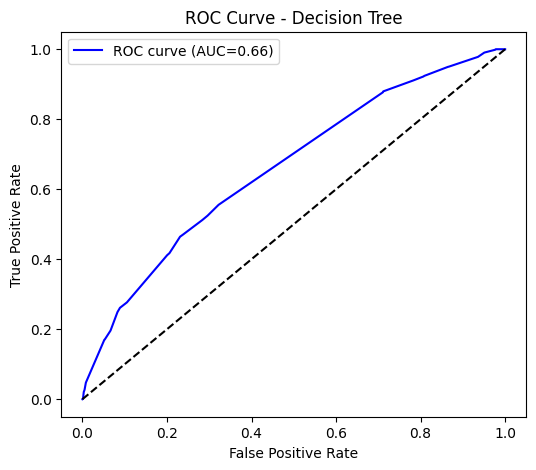
\includegraphics[width=0.45\textwidth]{images/rocDT.png}
    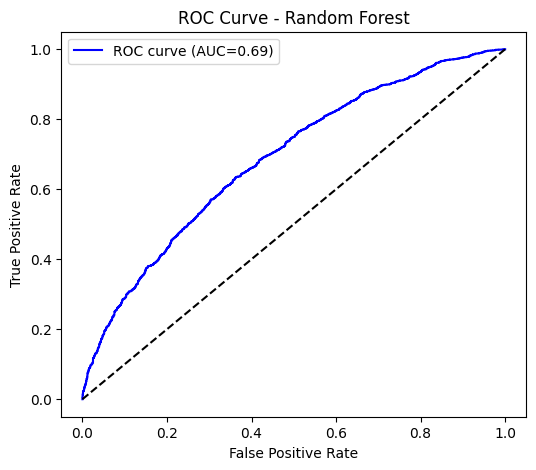
\includegraphics[width=0.45\textwidth]{images/rocRF.png}

    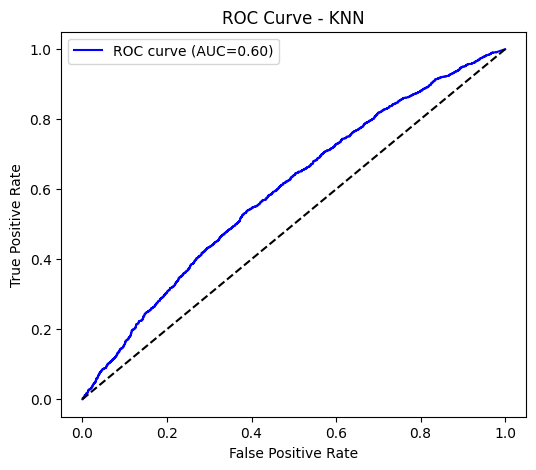
\includegraphics[width=0.45\textwidth]{images/rocKNN.png}
    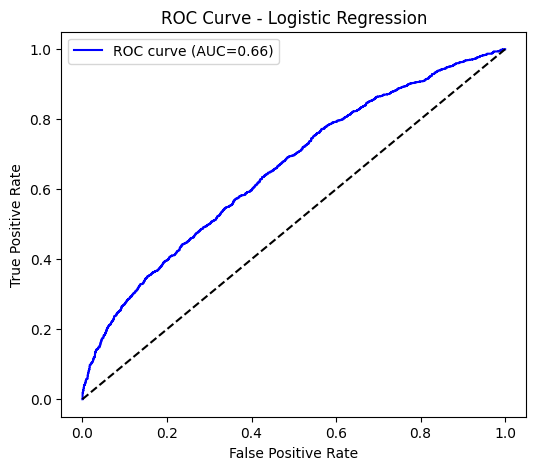
\includegraphics[width=0.45\textwidth]{images/rocLR.png}

    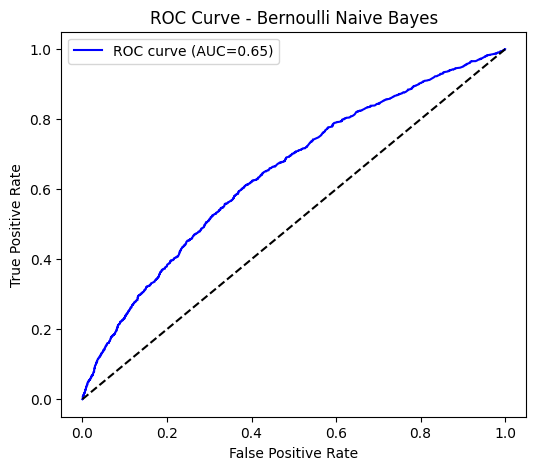
\includegraphics[width=0.6\textwidth]{images/rocNB.png}

    \caption{ROC curves of the models evaluated on the test set}
    \label{fig:cinque-immagini}
\end{figure}



\subsection{Feature Importances}

Table \ref{tab:top10_features_colored} shows the ten most important features as determined by the best model (Random Forest), along with their relative importance scores.

\begin{table}[ht]
\centering
\caption{Top 10 Features by Importance}
\label{tab:top10_features_colored}
\begin{tabular}{clc}
\toprule
\textbf{Rank} & \textbf{Feature} & \textbf{Importance} \\
\midrule
\rowcolor{red!40} 1  & number\_inpatient         & 0.2129 \\
\rowcolor{red!20} 2  & num\_lab\_procedures      & 0.0844 \\
\rowcolor{red!20} 3  & num\_medications          & 0.0833 \\
\rowcolor{red!20} 4  & discharge\_disposition\_id & 0.0808 \\
\rowcolor{orange!20} 5  & number\_diagnoses         & 0.0650 \\
\rowcolor{orange!20} 6  & number\_emergency         & 0.0549 \\
\rowcolor{orange!20} 7  & time\_in\_hospital        & 0.0540 \\
\rowcolor{orange!20} 8  & number\_outpatient        & 0.0528 \\
\rowcolor{yellow!20} 9  & admission\_source\_id     & 0.0461 \\
\rowcolor{yellow!20} 10 & num\_procedures           & 0.0389 \\
\bottomrule
\end{tabular}
\end{table}

\noindent
Analyzing the top-ranked features reveals several important insights into the factors influencing hospital readmission. In particular, the features highlighted in red indicate the strongest predictors:

\begin{itemize}
    \item \textbf{number\_inpatient} emerges as the single most influential factor, showing that patients with a higher number of prior hospitalizations face a substantially increased risk of readmission.
    \item \textbf{num\_lab\_procedures} and \textbf{num\_medications} reflect the clinical complexity and severity of a patient's condition, indicating that those requiring more tests or medications are more susceptible to returning to the hospital.
    \item \textbf{discharge\_disposition\_id} demonstrates that the type of discharge destination significantly impacts readmission risk, suggesting that patients discharged to environments with limited follow-up or support are more likely to be readmitted.
\end{itemize}
\noindent
\noindent
This suggests that both the patient's prior utilization of hospital services and the complexity of their current clinical condition play critical roles in predicting readmission. Overall, these findings highlight the importance of careful monitoring of high-risk patients and ensuring appropriate post-discharge follow-up in order to reduce readmission rates.

